% Krino v3 -- B2 marker-residual decision model
% Build: make build   (uses oaklight/texlive:science-cn)
\documentclass[tikz,border=10pt]{standalone}
\usepackage{amsmath}
\usepackage{amssymb}
\usetikzlibrary{arrows.meta,positioning,calc,decorations.pathreplacing,shapes.geometric}

% ---------------------------------------------------------------- palette
\definecolor{frozenfill}{HTML}{F3F4F6}
\definecolor{frozendraw}{HTML}{6B7280}
\definecolor{trainfill}{HTML}{EFF6FF}
\definecolor{trainraw}{HTML}{2563EB}
\definecolor{datafill}{HTML}{F0FDF4}
\definecolor{datadraw}{HTML}{16A34A}
\definecolor{fusefill}{HTML}{F5F3FF}
\definecolor{fusedraw}{HTML}{7C3AED}
\definecolor{lossfill}{HTML}{FFFBEB}
\definecolor{lossdraw}{HTML}{D97706}
\definecolor{markerfill}{HTML}{FEF2F2}
\definecolor{markerdraw}{HTML}{DC2626}
\definecolor{notefill}{HTML}{FAFAF9}

\tikzset{
  box/.style={rounded corners=3pt, draw, line width=0.6pt, align=center,
              inner sep=5pt, font=\sffamily\small},
  frozen/.style={box, fill=frozenfill, draw=frozendraw},
  trainable/.style={box, fill=trainfill, draw=trainraw},
  data/.style={box, fill=datafill, draw=datadraw},
  fusebox/.style={box, fill=fusefill, draw=fusedraw},
  lossbox/.style={box, fill=lossfill, draw=lossdraw},
  note/.style={rounded corners=3pt, draw=black!30, line width=0.5pt,
               fill=notefill, align=flush left, inner sep=5pt,
               font=\sffamily\footnotesize},
  token/.style={draw=frozendraw, fill=white, rounded corners=1.5pt,
                minimum height=0.5cm, inner sep=3pt, font=\sffamily\scriptsize},
  marker/.style={token, draw=markerdraw, fill=markerfill,
                 font=\sffamily\scriptsize\bfseries},
  arrow/.style={-{Stealth[length=2.2mm,width=1.6mm]}, line width=0.6pt,
                draw=black!70},
  dasharrow/.style={arrow, dashed},
  alabel/.style={font=\sffamily\scriptsize, text=black!65, align=center},
}

\begin{document}
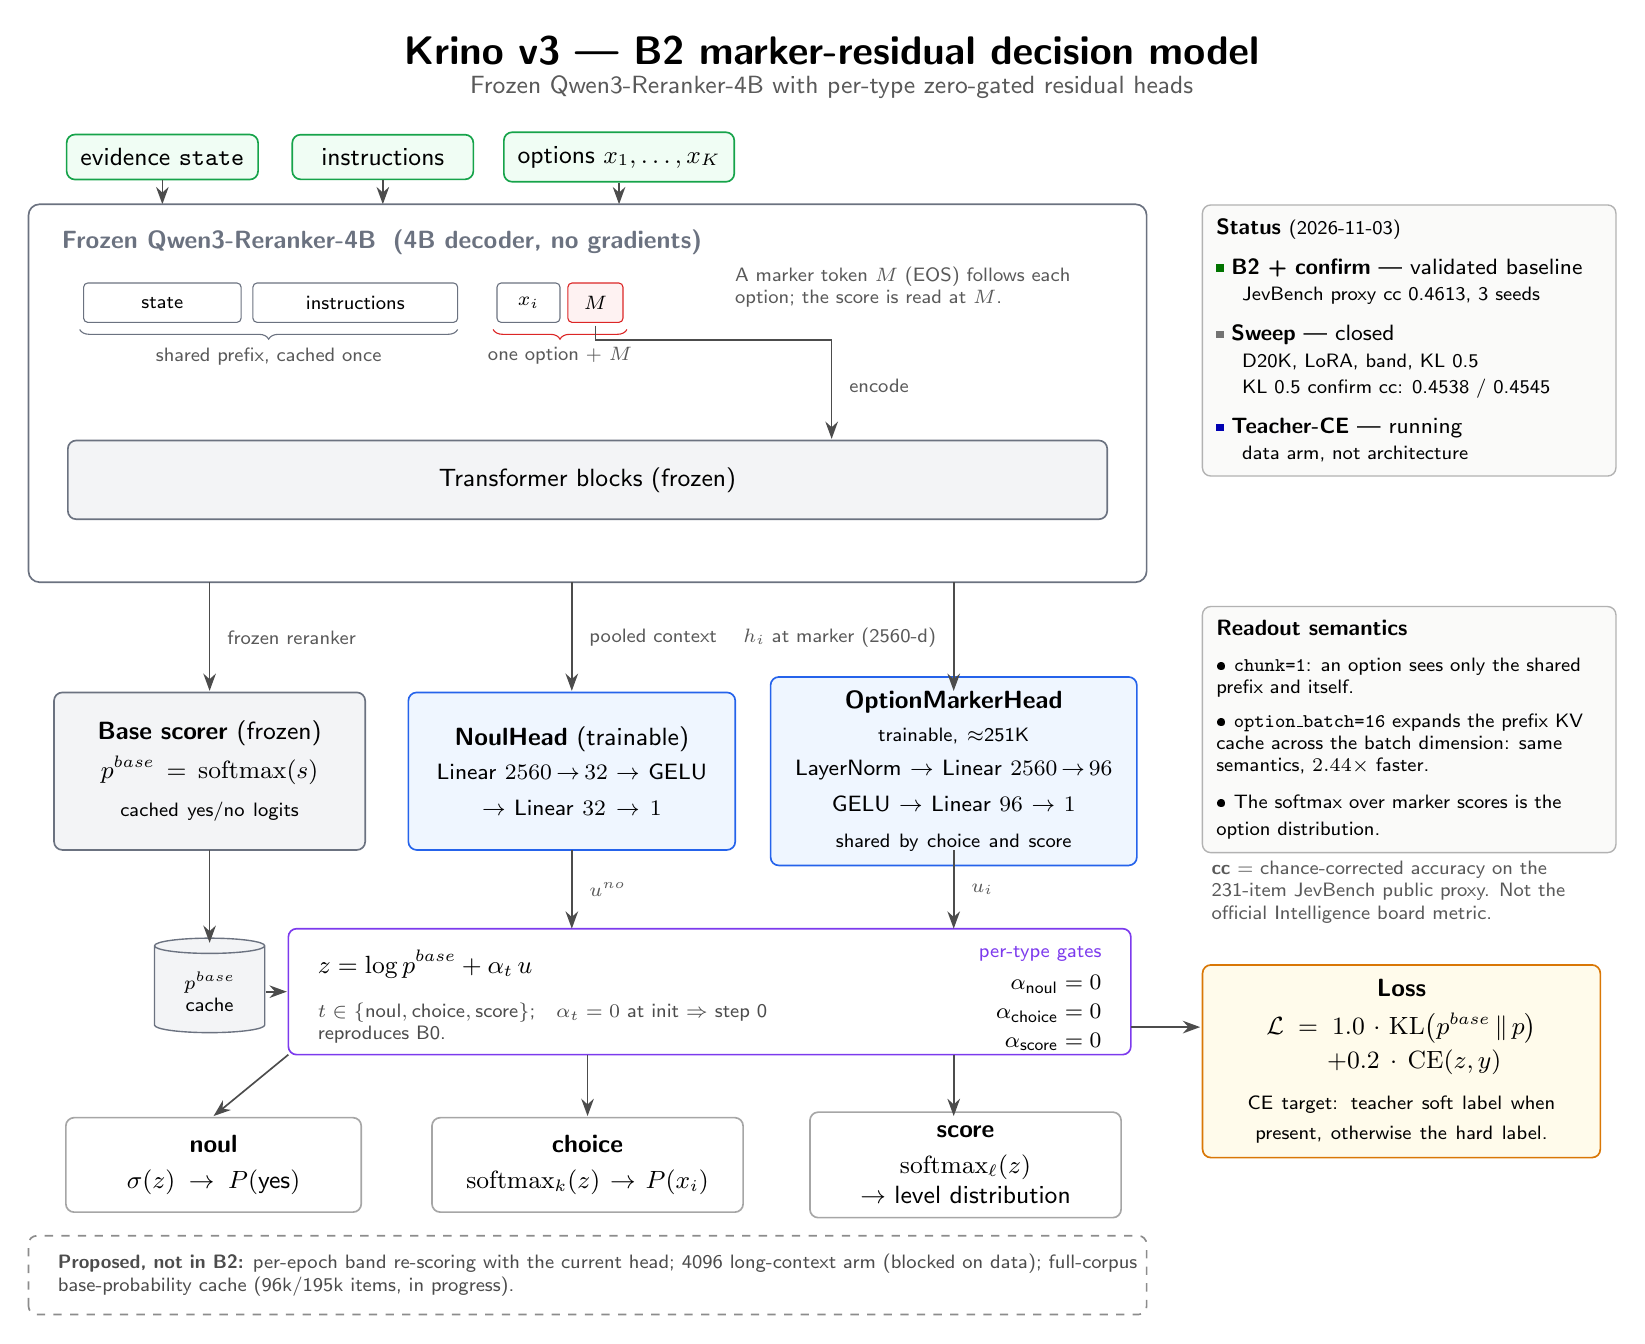
\begin{tikzpicture}[font=\sffamily]

% ================================================================ title
\node[font=\sffamily\Large\bfseries] at (10.6,16.35)
  {\textsf{Krino v3 --- B2 marker-residual decision model}};
\node[font=\sffamily\small, text=black!65] at (10.6,15.88)
  {\textsf{Frozen Qwen3-Reranker-4B with per-type zero-gated residual heads}};

% ================================================================ inputs
\node[data, minimum width=2.0cm] (instate) at (2.1,15.0) {evidence \texttt{state}};
\node[data, minimum width=2.3cm] (ininstr) at (4.9,15.0) {instructions};
\node[data, minimum width=2.6cm] (inopts)  at (7.9,15.0) {options $x_1,\dots,x_K$};
\foreach \n in {instate,ininstr,inopts}
  \draw[arrow] (\n.south) -- (\n.south |- 0,14.4);

% ================================================================ backbone
\draw[frozenfill, draw=frozendraw, line width=0.6pt, rounded corners=4pt]
  (0.4,9.6) rectangle (14.6,14.4);
\node[anchor=north west, font=\sffamily\small\bfseries, text=frozendraw]
  at (0.7,14.2) {Frozen Qwen3-Reranker-4B \;(4B decoder, no gradients)};

% token strip: shared prefix | option + marker
\node[token, minimum width=2.0cm] (tstate) at (2.1,13.15) {state};
\node[token, minimum width=2.6cm] (tinstr) at (4.55,13.15) {instructions};
\node[token, minimum width=0.8cm] (topt)   at (6.75,13.15) {$x_i$};
\node[marker, minimum width=0.7cm] (tmark) at (7.60,13.15) {$M$};

\draw[decorate, decoration={brace, amplitude=3.5pt, raise=2pt, mirror}, draw=frozendraw]
  (1.05,12.88) -- (5.85,12.88)
  node[midway, below=5pt, font=\sffamily\scriptsize, text=black!65]
  {shared prefix, cached once};
\draw[decorate, decoration={brace, amplitude=3.5pt, raise=2pt, mirror}, draw=markerdraw]
  (6.30,12.88) -- (8.00,12.88)
  node[midway, below=5pt, font=\sffamily\scriptsize, text=black!65]
  {one option + $M$};

\node[anchor=west, font=\sffamily\scriptsize, text=black!65, align=flush left,
      text width=4.6cm] at (9.25,13.35)
  {A marker token $M$ (EOS) follows each option; the score is read at $M$.};

% transformer blocks
\node[frozen, minimum width=13.2cm, minimum height=1.0cm] (blocks) at (7.5,10.9)
  {Transformer blocks (frozen)};
\draw[arrow] (7.60,12.86) -- (7.60,12.68) -- (10.60,12.68) -- (10.60,11.42);
\node[alabel, anchor=west] at (10.70,12.10) {encode};

% ================================================================ head row
\node[frozen, text width=3.6cm, minimum height=2.0cm] (base) at (2.70,7.20)
  {\textbf{Base scorer} (frozen)\\[3pt]
   $p^{base}=\operatorname{softmax}(s)$\\[3pt]
   {\scriptsize cached yes/no logits}};
\draw[arrow] (2.70,9.6) -- (2.70,8.22);
\node[alabel, anchor=west] at (2.80,8.90) {frozen reranker};

\node[trainable, text width=3.8cm, minimum height=2.0cm] (noulhead) at (7.30,7.20)
  {\textbf{NoulHead} (trainable)\\[3pt]
   {\footnotesize Linear $2560\!\to\!32\to$ GELU\\[2pt]
   $\to$ Linear $32\!\to\!1$}};
\draw[arrow] (7.30,9.6) -- (7.30,8.22);
\node[alabel, anchor=west] at (7.40,8.90) {pooled context};

\node[trainable, text width=4.3cm, minimum height=2.0cm] (markerhead) at (12.15,7.20)
  {\textbf{OptionMarkerHead}\\[1pt]
   {\scriptsize trainable, $\approx$251K}\\[3pt]
   {\footnotesize LayerNorm $\to$ Linear $2560\!\to\!96$\\[2pt]
   GELU $\to$ Linear $96\!\to\!1$}\\[2pt]
   {\scriptsize shared by choice and score}};
\draw[arrow] (12.15,9.6) -- (12.15,8.22);
\node[alabel, anchor=east] at (12.05,8.90) {$h_i$ at marker (2560-d)};

% ================================================================ p_base cache
\node[cylinder, draw=frozendraw, fill=frozenfill, line width=0.5pt,
      shape border rotate=90, aspect=0.22,
      minimum width=1.4cm, minimum height=1.2cm,
      font=\sffamily\scriptsize, align=center] (cache) at (2.70,4.40)
  {$p^{base}$\\cache};
\draw[arrow] (2.70,6.20) -- (2.70,5.02);

% ================================================================ fusion
\draw[fusefill, draw=fusedraw, line width=0.6pt, rounded corners=3pt]
  (3.70,3.60) rectangle (14.40,5.20);
\node[anchor=north west, font=\sffamily\small] at (3.95,5.05)
  {$\displaystyle z=\log p^{base}+\alpha_t\,u$};
\node[anchor=north west, font=\sffamily\scriptsize, text=black!70,
      text width=6.9cm, align=flush left] at (3.95,4.38)
  {$t\in\{\text{noul},\text{choice},\text{score}\}$;\quad
   $\alpha_t=0$ at init $\Rightarrow$ step 0 reproduces B0.};
\node[anchor=north east, font=\sffamily\footnotesize, align=right] at (14.15,5.10)
  {{\scriptsize\color{fusedraw}per-type gates}\\[2pt]
   $\alpha_{\text{noul}}=0$\\[1pt]$\alpha_{\text{choice}}=0$\\[1pt]$\alpha_{\text{score}}=0$};

\draw[arrow] (3.42,4.40) -- (3.68,4.40);
\draw[arrow] (7.30,6.20) -- (7.30,5.20);
\node[alabel, anchor=west] at (7.40,5.70) {$u^{no}$};
\draw[arrow] (12.15,6.20) -- (12.15,5.20);
\node[alabel, anchor=west] at (12.25,5.70) {$u_i$};

% ================================================================ outputs
\node[box, draw=black!35, fill=white, text width=3.4cm, minimum height=1.2cm]
  (outnoul) at (2.75,2.20)
  {\textbf{noul}\\[2pt] $\sigma(z)\to P(\text{yes})$};
\node[box, draw=black!35, fill=white, text width=3.6cm, minimum height=1.2cm]
  (outchoice) at (7.50,2.20)
  {\textbf{choice}\\[2pt] $\operatorname{softmax}_k(z)\to P(x_i)$};
\node[box, draw=black!35, fill=white, text width=3.6cm, minimum height=1.2cm]
  (outscore) at (12.30,2.20)
  {\textbf{score}\\[2pt] $\operatorname{softmax}_\ell(z)$\\ $\to$ level distribution};

\draw[arrow] (3.70,3.60) -- (2.75,2.82);
\draw[arrow] (7.50,3.60) -- (7.50,2.82);
\draw[arrow] (12.15,3.60) -- (12.15,2.82);

% ================================================================ metric note
\node[anchor=north west, font=\sffamily\scriptsize, text=black!65,
      text width=4.9cm, align=flush left] at (15.3,6.18)
  {\textbf{cc} = chance-corrected accuracy on the 231-item JevBench public
   proxy. Not the official Intelligence board metric.};

% ================================================================ loss
\node[lossbox, anchor=north west, text width=4.7cm] (loss) at (15.3,4.75)
  {\textbf{Loss}\\[3pt]
   $\mathcal{L}=1.0\cdot\mathrm{KL}\!\left(p^{base}\,\|\,p\right)$\\[1pt]
   $\quad+0.2\cdot\mathrm{CE}(z,y)$\\[4pt]
   {\scriptsize CE target: teacher soft label when present,
    otherwise the hard label.}};
\draw[arrow] (14.40,3.95) -- (15.28,3.95);

% ================================================================ status
\node[note, anchor=north west, text width=4.9cm] (status) at (15.3,14.4)
  {\textbf{Status} {\scriptsize(2026-11-03)}\\[5pt]
   \textcolor{green!45!black}{\rule[0.25ex]{0.75ex}{0.75ex}}
   \textbf{B2 + confirm} --- validated baseline\\
   \hspace*{1.1em}{\scriptsize JevBench proxy cc 0.4613, 3 seeds}\\[5pt]
   \textcolor{black!55}{\rule[0.25ex]{0.75ex}{0.75ex}}
   \textbf{Sweep} --- closed\\
   \hspace*{1.1em}{\scriptsize D20K, LoRA, band, KL 0.5}\\
   \hspace*{1.1em}{\scriptsize KL 0.5 confirm cc: 0.4538 / 0.4545}\\[5pt]
   \textcolor{blue!70!black}{\rule[0.25ex]{0.75ex}{0.75ex}}
   \textbf{Teacher-CE} --- running\\
   \hspace*{1.1em}{\scriptsize data arm, not architecture}};

% ================================================================ readout note
\node[note, anchor=north west, text width=4.9cm] (readout) at (15.3,9.30)
  {\textbf{Readout semantics}\\[5pt]
   {\scriptsize
   \textbullet\ \texttt{chunk=1}: an option sees only the shared
   prefix and itself.\\[4pt]
   \textbullet\ \texttt{option\_batch=16} expands the prefix KV cache
   across the batch dimension: same semantics, $2.44\times$ faster.\\[4pt]
   \textbullet\ The softmax over marker scores is the option
   distribution.}};

% ================================================================ proposed strip
\draw[dashed, draw=black!45, line width=0.6pt, rounded corners=3pt]
  (0.4,0.30) rectangle (14.6,1.30);
\node[anchor=west, font=\sffamily\scriptsize, text=black!70,
      text width=13.8cm, align=flush left] at (0.65,0.80)
  {\textbf{Proposed, not in B2:} per-epoch band re-scoring with the current head;
   4096 long-context arm (blocked on data); full-corpus base-probability cache
   (96k/195k items, in progress).};

\end{tikzpicture}
\end{document}
